\documentclass[a4paper,11pt]{article}
\usepackage[utf8]{inputenc}
\usepackage{graphicx}
\usepackage[hyphens]{url}
\usepackage[hidelinks]{hyperref}
\usepackage{tabularx}
\usepackage[centering, a4paper, margin=2.0cm, a4paper,]{geometry}
\usepackage[usenames,dvipsnames]{xcolor}
\usepackage{tikz} \usetikzlibrary{calc, arrows.meta, intersections, patterns, positioning, shapes.misc, fadings, through, decorations.pathreplacing}
\usepackage[utf8]{inputenc}
\usepackage{amsmath, amssymb, latexsym}
\usepackage{amsmath}
\usepackage{float}
\usepackage{eqexpl}
\eqexplSetDelim{=}
\eqexplSetIntro{where}
\usepackage{tikz}
\usetikzlibrary{decorations.pathreplacing}
\usetikzlibrary{fadings}
\usepackage{mathtools,amsfonts,amsthm}  % mathtools loads amsmath
\usepackage{placeins}
\usepackage{lipsum}

\definecolor{ColorOne}{named}{MidnightBlue}
\definecolor{ColorTwo}{named}{Dandelion}
\definecolor{ColorThree}{named}{Plum}
\definecolor{ColourFour}{named}{PineGreen}
\definecolor{ColourFive}{named}{OliveGreen}
%%%% modifying APS template a bit:
% times 
% \usepackage{mathptmx}
% arabic number section
% section left-side and title style
\usepackage{titlesec}
% spacing after and before section headers
\titlespacing*{\section}{0pt}{2.8ex plus 1ex minus .5ex}{2ex}
\titlespacing*{\subsection}{0pt}{2.2ex plus 1ex minus .5ex}{1.5ex}
\usepackage{natbib}
\definecolor{blueish2}{HTML}{0830Bb}
\hypersetup{colorlinks = true,
            linkcolor = blueish2,
            urlcolor  = blueish2,
            citecolor = black,
            anchorcolor = blueish2}
% section left-side and title style


\title{Borůvka's Algorithm}
% \author{NO AUTHORS GIVEN}
\author{Student Number: 700037512}
\date{}

\begin{document}

\maketitle
\thispagestyle{empty}
\begin{abstract}
\noindent

\end{abstract}

\vspace*{\fill}
\begin{center}
\noindent I certify that all material in this report which is not my own work has been
identified
\end{center}
\vspace{1em}

Signature: \hrulefill
\clearpage
\pagenumbering{arabic} 

\newpage
\section{Introduction}
In 1926 Otakar Borůvka published an algorithm to find the minimum spanning tree of a graph, it was the first of its kind and creating a minimum spanning tree has since become a classic problem with many different algorithmic solutions \cite{4392963}\cite{nevsetril2012origins}. A minimum spanning tree of an undirected graph $G(V,E)$, where V is the number of vertexes and E the number of edges, is the edges required to connect all the vertices for the lowest total edge cost without producing a cycle \cite{mst}. Figure 1 shows an example of a minimum spanning tree. 
\begin{figure}[!h]
    \centering
    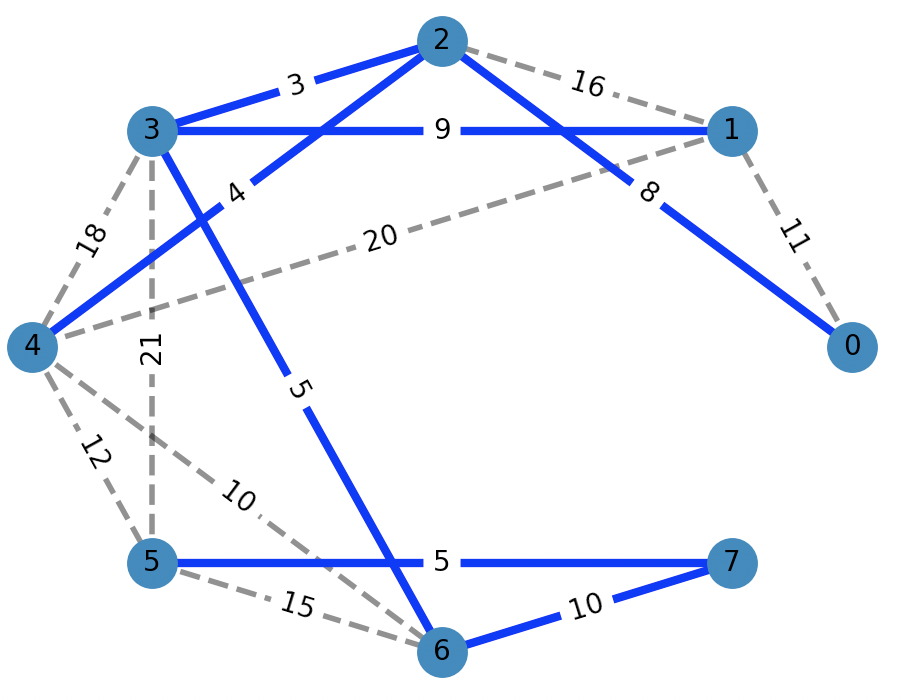
\includegraphics[width = 0.7\textwidth]{Screenshot 2022-12-07 at 5.26.26 pm.png}
    \caption{The minimum spanning tree of the graph is shown in blue. It connects all nodes together and contains no cycles.}
    \label{fig:my_label}
\end{figure}
\FloatBarrier
Minimum spanning trees are used in a range of applications such as designing telecommunication or other digital networks and travelling salesman problem \cite{nagarajan2014application}.
\section{Main Principles}

Borůvka's algorithm is a greedy algorithm, therefore, it selects the best option available at each step. The algorithm begins setting all the nodes as separate components. The smallest connecting edge to every component is added into the minimum spanning tree and the nodes that have been connected merge into one component. This will create small disjoint trees where each tree signifies a component that must be connected together to form the minimum spanning tree. The process of finding the smallest connecting node to each component continues until there is only one component containing all the nodes. The final remaining component is the minimum spanning tree.
\newpage
\section{Pseudo code}
\begin{verbatim}
    def Borůvka's algorithm
    input: A undirected weighted graph G(V,E)
    output: The minimum spanning tree of G(V,E)
    
    minimum_spanning_tree = []
    component_size = []
    for each vertex create a component containing only itself 
    and add 1 to the component_size list
    no_components = number of vertices
    while there is more than one component:
        for every edge y connecting 2 components a and b in G:
            let min_edge_a be the cheapest edge for a 
            if y is smaller than min_edge_a:
                set y as min_edge_a
            let min_edge_b be the cheapest edge for b
            if y is smaller than than min_edge_b:
                set y as min_edge_b
        for every vertex in G:
            if cheapest_edge for components is not null:
                join the start (a) and the end (b) components together
                add cheapest_edge to minimum_spanning_tree
                no_components = no_components - 1

\end{verbatim}

\section{Complexity}

\section{Limitations}

\section{Applications}
\bibliographystyle{IEEEtran}
\bibliography{references}
\end{document}
